\documentclass[resume]{subfiles}


\begin{document}
\section{Fonctions de transfert}
\subsection{Marge de gain / marge de phase}
\begin{figure}[H]
\centering
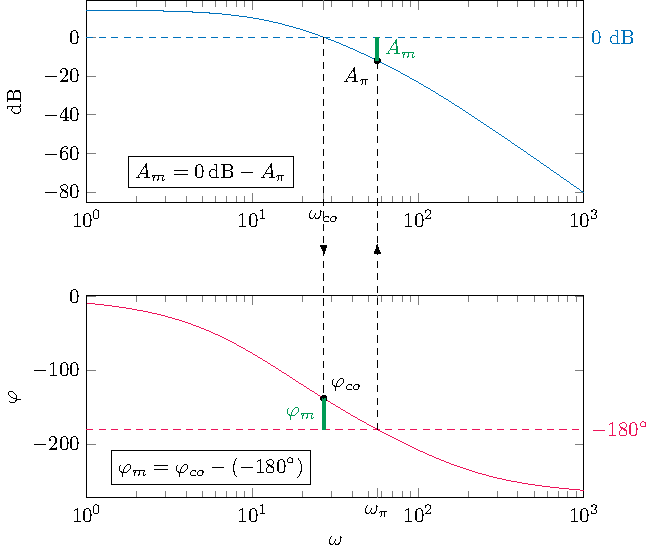
\includegraphics[width=\columnwidth]{drwg_4.pdf}
\end{figure}
\subsection{Équations aux différences}
\label{sec_eq_diff}
$$\LARGE \underset{\text{degré relatif}}{d}=\underset{\deg(\text{denominateur})}{n}-\underset{\deg(\text{numérateur})}{m}$$
Forme développée ($Y$ en fonction de $U$)
\begin{multline*}
Y(z)\left(\textcolor{Gray}{a_0=1}+\acolor{a_1}z^{-1}+\acolor{a_2}z^{-2}+\cdots+\acolor{a_n}z^{-n}\right)=\\U(z)\left(\bcolor{b_0}z^{-d}+\bcolor{b_1}z^{-d-1}+\bcolor{b_2}z^{-d-2}+\cdots+\bcolor{b_m}z^{-d-m}\right)
\end{multline*}
Forme fonction de transfert avec puissances de $z$ négatives
On peut aussi écrire sous la forme $z^{-x}$
$$G(z)=\frac{\bcolor{b_0}z^{-d}+\bcolor{b_1}z^{-d-1}+\bcolor{b_2}z^{-d-2}+\cdots+\bcolor{b_m}z^{-d-m}}{\textcolor{Gray}{a_0}+\acolor{a_1}z^{-1}+\acolor{a_2}z^{-2}+\cdots+\acolor{a_n}z^{-n}}$$
$$G(z)=\frac{Y(z)}{U(z)}$$


\subsection{Normes d'une fonction de transfert}

\subsubsection{Norme 2}

$$
||G_2|| = \sqrt{\frac{1}{2\pi}\int_{-\infty}^{\infty}|G(j\omega)| d\omega}=$$
$$\sqrt{\int_{0}^{\infty}|g(t)| dt} = ||g||_2$$

\subsubsection{Norme $\infty$}

$$
||G||_{\infty} = max_{\omega}|G(j\omega)| = max_{u} \frac{||y||_2}{||u||_2}
$$

\subsection{Fonction de base}

<img src="FiguresTypora/image-20220519101441493.png" alt="image-20220519101441493" style="zoom: 33%;" />
le 'gang' cours 12 page 7

<img src="FiguresTypora/image-20220602091113238.png" alt="image-20220602091113238" style="zoom:33%;" />
allure typique cours 12 page 9

\subsection{Distance critique}

$$d_{crit} = min_{\omega}\{dist(L(j\omega)), -1\}$$
$$d_{crit} = min_{\omega}|1+L(j\omega)|$$
$$d_{crit} = \frac{1}{min_{\omega}|\frac{1}{1+L(j\omega)}|}$$
$$d_{crit} = \frac{1}{||S||_\infty}$$

\subsubsection{marge de phase et de gain}
$$A_m > \frac{1}{1-d_{crit}}$$
$$\varphi_m > 2\arcsin(\frac{d_{crit}}{2})$$

\end{document}